\documentclass{article}
\usepackage[utf8]{inputenc}
\usepackage[english,russian]{babel}
\usepackage{graphics}
\usepackage{amsmath}
\usepackage{indentfirst}
\usepackage{misccorr}
\usepackage{amsmath}
\usepackage{graphicx}
\graphicspath{{./pic/}}

\begin{document}


	Постройте график функции\\
	\begin{equation*}
	y(x) = 
	\begin{cases}
	\frac{5}{x} &\text{если $x < -1$}\\
	-x^2+4x &\text{если $x \ge -1$}\\
	\end{cases}
	\end{equation*}
	и определите, при каких значениях c  прямая {$y=c$}   будет пересекать построенный график в трёх точках.\\
	\graphicspath{{Pictures/}}
	\DeclareGraphicsExtensions{.pdf,.png,.jpg}
	\begin{figure}[hb]
		\begin{center}
			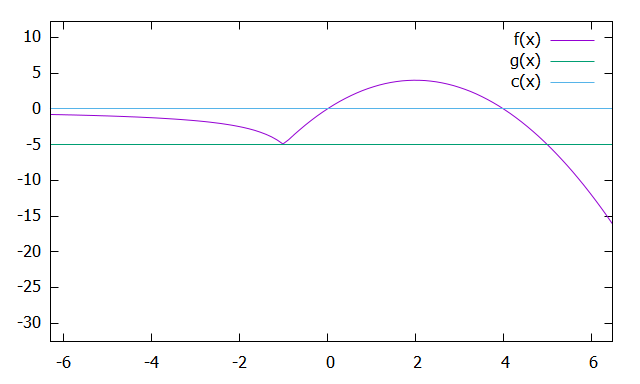
\includegraphics[scale=0.5]{Graphic}
		\end{center}
	\end{figure}
	\\
	\\
	1) При {$c<-5$} график  {$y=c$} будет пересекать график f(x) только в одной точке\\
	2) При {$c \geq 0$}  график  {$y=c$} будет пересекать график f(x) в одной точке, в двух точках или не будет пересекать вовсе\\
	3)При {$c \in [-5;0)$} график  {$y=c$} будет пересекать график f(x) только в трёх точках\\
	Ответ: {$c \in [-5;0)$}
	
\end{document}
